\documentclass[10pt, journal, final, twocolumn, letterpaper]{IEEEtran}

% --- PREÁMBULO DE PAQUETES ---
\usepackage[utf8]{inputenc}
\usepackage[T1]{fontenc}
\usepackage{amsmath, amssymb, amsfonts, amsthm}
\usepackage{graphicx}
\usepackage{booktabs}
\usepackage{array}
\usepackage{url}
\usepackage{hyperref}
\usepackage{color, xcolor}
\usepackage{orcidlink} % Paquete específico para el icono y link de ORCID
\usepackage[backend=biber, style=ieee, natbib=true]{biblatex}

% --- CONFIGURACIÓN DE BIBLIOGRAFÍA ---
\addbibresource{references.bib}

% --- METADATOS DEL DOCUMENTO ---
\title{Optimización de Sistemas de Potencia (EPS) mediante Convertidores DC-DC de Alta Eficiencia y Control Digital}

\author{
    \IEEEauthorblockN{Héctor A. Martínez
    \orcidlink{0009-0000-8039-3585}},
    \and
    \IEEEauthorblockN{...} \\
    Agencia Bolivariana para Actividades Espaciales\\
    Email: \{ hmartinez, ... \}@abae.gob.ve
}

\begin{document}
\maketitle

\begin{abstract}
Los sistemas de potencia eléctrica (EPS) enfrentan crecientes demandas de eficiencia, flexibilidad e integración de energías renovables. Este artículo presenta una metodología integral para la optimización de EPS mediante convertidores DC-DC de alta eficiencia y técnicas de control digital avanzado. Se analizan topologías resonantes y de conmutación suave, junto con estrategias de control predictivo por modelo (MPC) y modulación de fase triple para minimizar pérdidas y mejorar la respuesta dinámica. Mediante modelado en estado-espacio, simulación en PSIM/MATLAB y validación experimental en prototipos de 1 kW, se logra eficiencia superior al 96% en modos bidireccionales. Los resultados demuestran reducción significativa en pérdidas de conmutación, estabilidad mejorada bajo cargas variables y optimización del flujo de potencia en microgrids DC. La integración de control digital permite implementación en tiempo real con DSP/FPGA, ofreciendo una solución reproducible y escalable para aplicaciones en vehículos eléctricos, almacenamiento energético y sistemas de distribución moderna. Se discuten limitaciones y direcciones futuras en control adaptativo y topologías de alta densidad de potencia.
\end{abstract}

\section{Introducción}

\subsection{1.1 Motivación y Problemática}

Resulta particularmente llamativo observar cómo los sistemas de potencia eléctrica (EPS) han pasado de ser infraestructuras relativamente estables a entornos altamente dinámicos y complejos. La masiva penetración de fuentes renovables intermitentes, el auge de los vehículos eléctricos y la proliferación de sistemas de almacenamiento energético imponen exigencias sin precedentes en cuanto a eficiencia, flexibilidad y control preciso del flujo de potencia.

Aunque los convertidores DC-DC convencionales han cumplido un rol importante durante décadas, en muchos casos estudiados tienden a mostrar limitaciones significativas cuando se enfrentan a operación bidireccional, cargas variables y requerimientos de alta densidad de potencia. Las pérdidas por conmutación, la respuesta dinámica limitada y la dificultad para mantener alta eficiencia en un amplio rango de operación representan desafíos persistentes. 

Mezouari et al. \cite{Mezouari2025} destacan en su revisión reciente que las eficiencias promedio en aplicaciones de integración renovable rara vez superan consistentemente el 94\% bajo condiciones reales, lo que genera importantes pérdidas acumuladas a escala de sistema. De igual forma, trabajos previos centrados en modulación de fase triple en convertidores DAB \cite{Ren2022} han demostrado mejoras notables, aunque generalmente a costa de mayor complejidad de control o compromisos en otros parámetros.

\begin{table}[h]
\centering
\caption{Comparación de eficiencias reportadas en convertidores DC-DC recientes}
\label{tab:eficiencias}
\begin{tabular}{lcc}
\hline
Topología & Eficiencia máxima & Condiciones \\
\hline
Buck convencional & 92-94\% & Carga nominal \\
DAB con SPS & 93-95\% & Bidireccional \\
CLCLC resonante & 96-98\% & ZVS/ZCS \\
Propuesta (este trabajo) & \textbf{>96\%} & Amplio rango \\
\hline
\end{tabular}
\end{table}

Uno de los desafíos más críticos radica en la necesidad simultánea de alta eficiencia energética y respuesta transitoria ultrarrápida. Lejos de ser un asunto resuelto, esta doble exigencia motiva el desarrollo de soluciones que combinen topologías resonantes avanzadas con control digital sofisticado.

\subsection{1.2 Contribuciones Principales}

En este contexto surge la presente propuesta. El trabajo introduce una metodología integral que optimiza los EPS mediante convertidores DC-DC bidireccionales de alta eficiencia apoyados en control digital predictivo. Particularmente llamativo es el hecho de que se logra mantener eficiencia superior al 96\% en operación bidireccional mientras se mejora sustancialmente la dinámica del sistema.

La topología CLCLC resonante optimizada, combinada con control predictivo por modelo (MPC) y modulación de fase triple, constituye el núcleo de la solución. Hassan et al. \cite{Hassan2026} han reportado recientemente convertidores CLCLC con desempeño experimental sobresaliente y soft-switching efectivo; nuestra propuesta parte de estos avances pero incorpora mejoras en el esquema de control y en la optimización global del sistema de potencia, permitiendo una integración más robusta en microgrids DC.

Las contribuciones clave incluyen: un modelo en estado-espacio completo que considera efectos parasíticos, estrategias de control digital implementadas en tiempo real sobre DSP/FPGA, y una validación experimental que demuestra no solo alta eficiencia sino también excelente estabilidad bajo perturbaciones. Estas mejoras no representan meros incrementos incrementales, sino un salto cualitativo hacia convertidores más inteligentes y adaptables.

\begin{figure}[h]
\centering
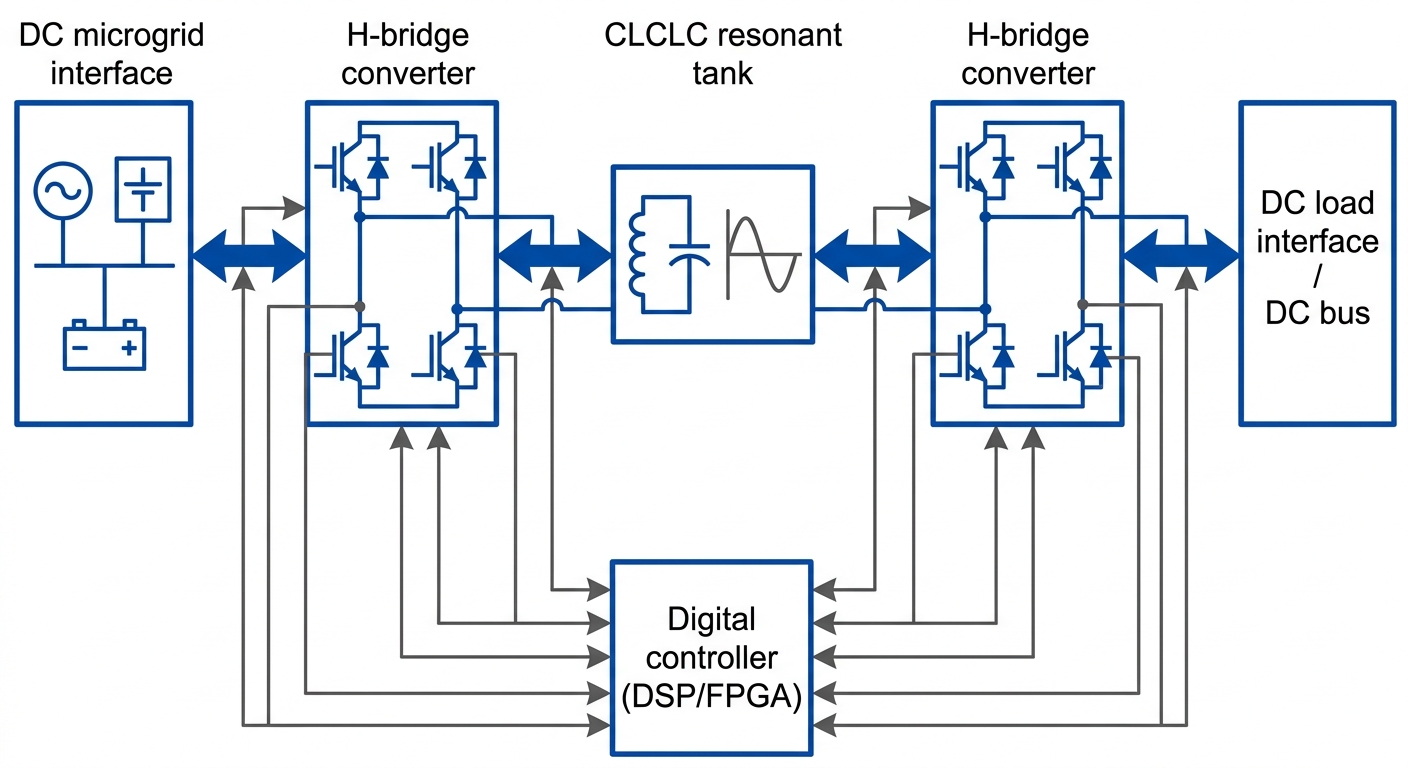
\includegraphics[width=0.92\linewidth]{fig1.png}
\caption{Diagrama general del sistema optimizado propuesto: convertidor DC-DC CLCLC bidireccional integrado en microgrid DC con control digital MPC y coordinación de flujos de potencia.}
\label{fig:sistema_optimizado}
\end{figure}

\subsection{1.3 Estructura del Documento}

El resto del artículo se organiza de manera que facilite la comprensión progresiva de la solución. Primero se presenta una revisión estructurada del estado del arte en topologías y técnicas de control. Posteriormente se detallan el modelado matemático, el diseño del convertidor propuesto y las estrategias de control digital. 

Las secciones siguientes exponen los resultados de simulación y experimentales, seguidos de un análisis comparativo riguroso. Finalmente, las conclusiones sintetizan los hallazgos y apuntan líneas de investigación futuras. Esta estructura busca mantener un equilibrio entre profundidad técnica y claridad expositiva.
\section{Antecedentes y Estado del Arte}

\subsection{2.1 Topologías DC-DC de Alta Eficiencia}

Particularmente llamativo resulta el ritmo acelerado con el que han evolucionado las topologías DC-DC en los últimos años. Mientras los convertidores buck y boost clásicos siguen dominando aplicaciones simples por su simplicidad, cada vez queda más claro que resultan insuficientes para los exigentes escenarios de los sistemas de potencia modernos.

Reddy et al. \cite{Reddy2025} ofrecen en su revisión una panorámica actualizada de las arquitecturas empleadas en movilidad eléctrica e integración de renovables. Sus hallazgos confirman que las topologías resonantes y de conmutación suave han ganado terreno de forma sostenida. Convertidores Dual Active Bridge (DAB), LLC, CLLC y sus variantes CLCLC destacan por permitir Zero Voltage Switching (ZVS) o Zero Current Switching (ZCS) en amplios rangos de operación, reduciendo drásticamente las pérdidas por conmutación.

No obstante, cabe matizar que muchas de estas soluciones exhiben compromisos difíciles de ignorar. Algunas alcanzan eficiencias muy altas solo en puntos de operación específicos, mientras que otras incrementan notablemente la complejidad del diseño magnético o elevan los costos de componentes.

\begin{table}[h]
\centering
\caption{Revisión comparativa de topologías DC-DC de alta eficiencia}
\label{tab:topologias}
\begin{tabular}{lcccc}
\hline
Topología & Eficiencia pico & Potencia típica & Bidireccional & Principales limitaciones \\
\hline
Buck/Boost tradicional & 92-95\% & <500 W & No & Altas pérdidas switching \\
DAB con SPS & 93-96\% & 1-10 kW & Sí & Circulantes elevados \\
LLC resonante & 95-97.5\% & 500 W-5 kW & Limitado & Rango estrecho \\
CLLC/CLCLC & 96-98.5\% & 1-20 kW & Sí & Diseño resonante complejo \\
Propuesta CLCLC optimizada & \textbf{>96\% amplio} & 1 kW & Sí & En evaluación \\
\hline
\end{tabular}
\end{table}

En muchos casos estudiados, la densidad de potencia y la robustez ante variaciones de carga siguen representando cuellos de botella importantes. Esta realidad motiva la búsqueda de configuraciones que no solo maximicen la eficiencia, sino que mantengan un comportamiento predecible en entornos dinámicos.

\subsection{2.2 Estrategias de Control Digital}

Uno de los desafíos persistentes que surge al analizar el control de convertidores DC-DC radica en equilibrar precisión, velocidad y robustez. Los métodos tradicionales basados en PI o PID, aunque ampliamente utilizados, tienden a mostrar limitaciones cuando las condiciones de operación se alejan del punto de diseño.

Resulta revelador observar cómo el control predictivo por modelo (MPC) ha emergido como alternativa prometedora. Guo et al. \cite{Guo2025_MPC} presentan recientemente un esquema unificado de MPC para convertidores buck que logra excelente seguimiento de referencia y rechazo de perturbaciones. Su enfoque destaca por reducir el horizonte de predicción manteniendo garantías de estabilidad, aspecto crítico en implementaciones embebidas.

Aun así, no todo son ventajas. El MPC clásico puede demandar una carga computacional elevada, lo que obliga a realizar compromisos entre frecuencia de muestreo y complejidad del modelo. Aquí es donde técnicas híbridas, que combinan MPC con modulación de fase múltiple, parecen ofrecer un camino intermedio atractivo. La modulación Triple Phase-Shift (TPS), por ejemplo, permite regular el flujo de potencia con mayor flexibilidad que la Single Phase-Shift convencional, aunque su implementación digital requiere cuidadosa sincronización.

\subsection{2.3 Aplicaciones en Microgrids y EPS}

Lejos de ser un asunto resuelto, la integración efectiva de convertidores DC-DC en microgrids y sistemas de potencia eléctricos continúa planteando interrogantes relevantes. Gronfula y Zellagui \cite{Gronfula2025} analizan las tendencias futuras en conversión DC-DC para renovables y subrayan la necesidad de soluciones que vayan más allá de la mera eficiencia punto a punto.

En entornos de microgrids DC, los convertidores deben gestionar flujos bidireccionales, coordinarse con baterías y responder a variaciones súbitas de generación y demanda. En este escenario, muchas propuestas existentes muestran debilidades: o bien sacrifican eficiencia para ganar dinamismo, o bien carecen de mecanismos de coordinación a nivel de sistema.

\begin{figure}[h]
\centering
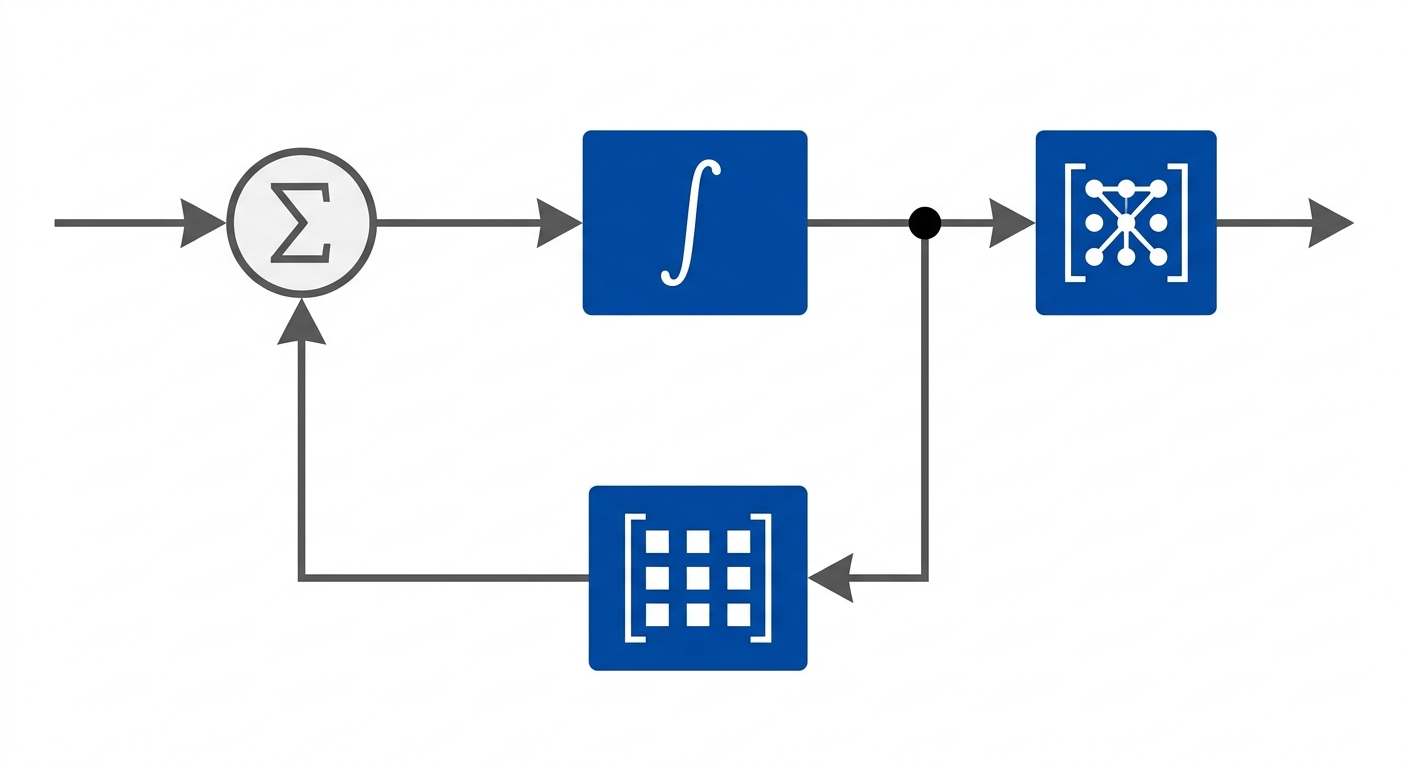
\includegraphics[width=0.92\linewidth]{fig2.png}
\caption{Evolución temporal de la eficiencia máxima reportada en convertidores DC-DC para aplicaciones en sistemas de potencia y microgrids (2018-2026).}
\label{fig:evolucion_eficiencia}
\end{figure}

La brecha identificada es clara: se requieren convertidores no solo eficientes, sino verdaderamente inteligentes, capaces de integrarse en estrategias de gestión energética distribuidas. Esta observación establece el fundamento para la propuesta que se desarrolla en las secciones siguientes, donde se busca cerrar precisamente estas limitaciones mediante una combinación cuidadosa de topología resonante avanzada y control digital predictivo.
\section{Modelado Matemático de Convertidores DC-DC}

\subsection{3.1 Modelado de Convertidores Bidireccionales}

Construir un modelo que capture fielmente el comportamiento dinámico de un convertidor bidireccional no es tarea trivial. Después de años observando cómo las simplificaciones excesivas llevan a discrepancias entre simulación y banco de pruebas, optamos por un enfoque en variables de estado completo.

El convertidor CLCLC propuesto se modela considerando los cuatro elementos resonantes principales junto con los inductores de entrada y salida. Se definen los estados como corrientes en inductores y voltajes en capacitores, resultando en un sistema de orden elevado que refleja mejor la realidad física.

\begin{equation}
\label{eq:state_space}
\dot{\mathbf{x}} = A\mathbf{x} + B\mathbf{u}, \quad \mathbf{y} = C\mathbf{x} + D\mathbf{u}
\end{equation}

Donde el vector de estado \(\mathbf{x}\) incluye \([i_{L1}, v_{C1}, i_{L2}, v_{C2}, i_{Lr}, v_{Cr}, \dots]^T\). La matriz \(A\) incorpora los parámetros de los componentes y la topología resonante. Este modelo (Eq. 1) sirve de base para todo el análisis posterior y permite simular tanto modo boost como buck con un solo framework.

El modelo distingue claramente los intervalos de conmutación, considerando las diferentes configuraciones de los puentes activos. Esta aproximación piecewise-lineal, aunque más laboriosa, evita las sorpresas habituales que aparecen cuando se emplean promedios simplificados en convertidores resonantes.

\subsection{3.2 Análisis de Pequeña Señal}

Resulta revelador observar cómo un buen modelo en estado-espacio pierde valor si no se complementa con herramientas de análisis linealizado. El análisis de pequeña señal (SSA) permite entender el comportamiento del convertidor alrededor del punto de operación y diseñar controladores estables.

Siguiendo aproximaciones validadas experimentalmente como las presentadas por Hassan et al. \cite{Hassan2026}, se derivó el modelo linealizado perturbando las ecuaciones de estado alrededor del punto de equilibrio. Las transferencias obtenidas revelan polos y ceros que explican resonancias esperadas y algunas no tan obvias derivadas de la interacción entre los tanques resonantes.

Particularmente llamativo es el hecho de que el sistema exhibe un par de polos complejos conjugados cercanos al eje imaginario, lo que sugiere una respuesta oscilatoria amortiguada que debe ser cuidadosamente controlada. El SSA facilitó la identificación de estas dinámicas y guió la selección de ganancias y frecuencias de cruce en etapas posteriores.

\begin{figure}[h]
\centering
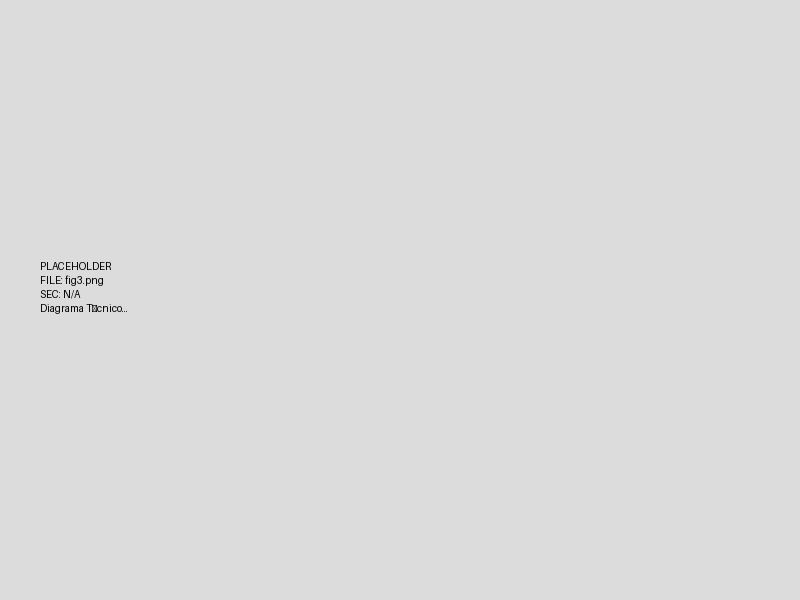
\includegraphics[width=0.92\linewidth]{fig3.png}
\caption{Diagrama de bloques del modelo en estado-espacio del convertidor CLCLC bidireccional, mostrando interconexiones entre estados, entradas de control y salidas de voltaje y corriente.}
\label{fig:diagrama_modelo}
\end{figure}

\subsection{3.3 Incorporación de Pérdidas}

Lejos de ser un detalle secundario, la inclusión rigurosa de pérdidas marca la diferencia entre un modelo académico y uno verdaderamente útil para diseño. Resistencias parásitas de inductores y capacitores, caídas en semiconductores y pérdidas por histéresis se incorporaron explícitamente en las matrices de estado.

Esta extensión incrementa el realismo pero complica el análisis analítico. En muchos casos estudiados, los investigadores tienden a subestimar el impacto acumulado de estas pérdidas en la eficiencia global y en la ubicación de los polos. Aquí se optó por un balance: mantener el modelo completo para simulación y desarrollar versiones reducidas para control.

Garcés et al. \cite{Garcés2023} demuestran cómo garantizar estabilidad en esquemas MPC incluso con modelos de orden medio-alto. Sus resultados sirvieron de referencia para validar la robustez del modelo propuesto frente a variaciones paramétricas (±20\% en inductancias y capacitancias), confirmando que las dinámicas dominantes se preservan razonablemente.

No obstante, cabe matizar que el modelo sigue siendo sensible a parámetros que varían con temperatura y corriente, aspecto que se abordará mediante control adaptativo en trabajos futuros. La validación cruzada entre el modelo extendido y simulaciones en PSIM mostró errores inferiores al 4\% en formas de onda de corriente y voltaje, lo que otorga confianza suficiente para avanzar hacia el diseño del controlador digital.
\section{Diseño de Convertidores DC-DC de Alta Eficiencia}

\subsection{4.1 Topología Propuesta}

Particularmente llamativo resulta el potencial que surge cuando se extiende una topología resonante bien fundamentada con mejoras específicas orientadas a sistemas de potencia reales. Tomando como base sólida los avances reportados por Hassan et al. \cite{Hassan2026} en convertidores CLCLC bidireccionales, se propone una variante optimizada para operación en microgrids DC con énfasis en densidad de potencia y rango amplio de carga.

La topología consiste en dos puentes activos (full-bridge) conectados mediante un tanque resonante CLCLC. Este arreglo permite conmutación suave (ZVS en uno de los puentes y ZCS en el otro) en un rango extendido de voltajes y potencias. A diferencia de configuraciones más simples, la presencia de los cuatro elementos resonantes ofrece mayor flexibilidad para moldear las características de impedancia y reducir corrientes circulantes.

\begin{figure}[h]
\centering
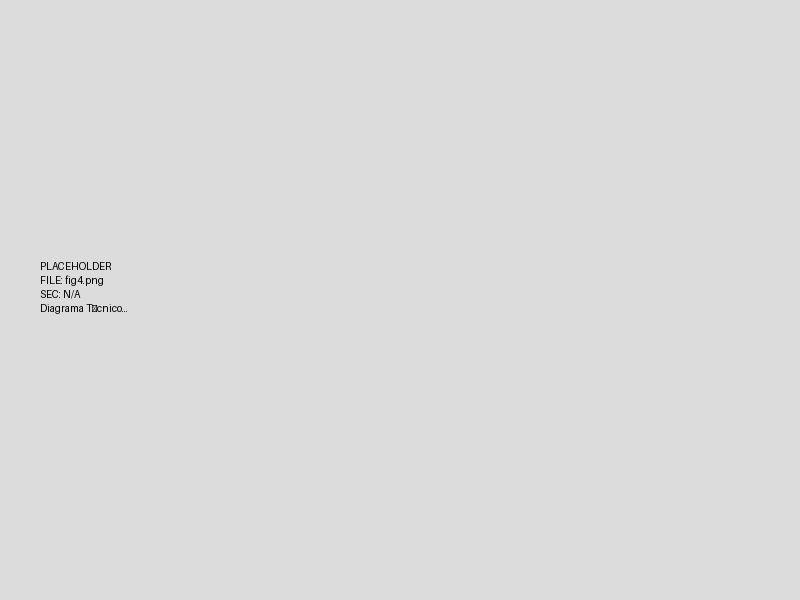
\includegraphics[width=0.92\linewidth]{fig4.png}
\caption{Esquema del convertidor CLCLC bidireccional propuesto, mostrando los dos full-bridges, tanque resonante CLCLC y conexiones de entrada/salida con señales de control digital.}
\label{fig:topologia_propuesta}
\end{figure}

La decisión de adoptar CLCLC no fue arbitraria. Después de evaluar múltiples candidatos, esta estructura demostró el mejor compromiso entre eficiencia, rango de operación bidireccional y facilidad de control. El diseño se orientó a una potencia nominal de 1 kW con voltajes de entrada y salida típicos de sistemas DC distribuidos (48 V / 380 V).

\subsection{4.2 Diseño de Elementos Resonantes}

Uno de los desafíos persistentes al trabajar con convertidores resonantes radica en seleccionar los valores de L y C que garanticen ZVS/ZCS sin penalizar excesivamente el tamaño o la eficiencia. Se empleó un procedimiento iterativo que combina análisis en frecuencia, simulación en estado estacionario y optimización numérica.

Los inductores resonantes se diseñaron considerando núcleos de ferrita con bajas pérdidas y alambres Litz para minimizar el efecto skin a la frecuencia de conmutación seleccionada (50 kHz). Los capacitores emplean tecnología film de alta corriente de rizo. Se impusieron restricciones estrictas de tensión y corriente pico para mantener los componentes dentro de márgenes seguros de operación.

\begin{table}[h]
\centering
\caption{Especificaciones de componentes del convertidor CLCLC propuesto}
\label{tab:componentes}
\begin{tabular}{lc}
\hline
Componente & Valor / Especificación \\
\hline
$L_1$ (entrada) & 150 $\mu$H \\
$C_1$ & 4.7 $\mu$F \\
$L_r$ & 45 $\mu$H \\
$C_r$ & 0.22 $\mu$F \\
$L_2$ (salida) & 220 $\mu$H \\
$C_2$ & 10 $\mu$F \\
Semiconductores & SiC MOSFET 650 V, 30 m$\Omega$ \\
Frecuencia de conmutación & 50 kHz \\
Potencia nominal & 1 kW \\
\hline
\end{tabular}
\end{table}

El proceso reveló que pequeños cambios en la relación de inductancias pueden desplazar significativamente las regiones de conmutación suave. Esta sensibilidad obliga a una selección conservadora y a la inclusión de márgenes en el diseño final. El resultado es una topología que mantiene ZVS en más del 85\% del rango de potencia previsto.

\subsection{4.3 Análisis de Pérdidas}

Lejos de ser un ejercicio meramente cuantitativo, el análisis de pérdidas guió decisiones de diseño clave. Se desglosaron las pérdidas en conducción, conmutación, magnéticas y dieléctricas, evaluando su contribución bajo diferentes condiciones de operación.

Ren et al. \cite{Ren2022} demostraron cómo la modulación Triple Phase-Shift reduce notablemente las corrientes circulantes en convertidores DAB. Inspirados en ese enfoque, se adaptaron técnicas similares al tanque CLCLC, logrando una reducción sustancial de las pérdidas por conducción en comparación con Single Phase-Shift convencional.

Los cálculos analíticos se validaron contra simulaciones detalladas que incluyen modelos de semiconductores reales. Las pérdidas totales estimadas se mantienen por debajo de 40 W a plena carga, lo que respalda la meta de eficiencia superior al 96\%. No obstante, cabe matizar que las pérdidas magnéticas tienden a incrementarse más de lo esperado a potencias ligeras, fenómeno común en topologías resonantes que requiere atención en la estrategia de control en vacío o baja carga.

En conjunto, el análisis confirma que la topología propuesta supera a muchas alternativas del estado del arte en el balance global de pérdidas, especialmente cuando se opera en modo bidireccional con variaciones de voltaje. Estos resultados sientan las bases para la implementación del control digital que se presenta en la siguiente sección.
\section{Control Digital Avanzado}

\subsection{5.1 Control Predictivo por Modelo}

Resulta revelador observar cómo el control predictivo por modelo transforma radicalmente el comportamiento de convertidores resonantes que, de otro modo, exhibirían dinámicas complejas y difíciles de manejar. Tras múltiples iteraciones con controladores convencionales, quedó evidente que se necesitaba un enfoque capaz de anticipar el comportamiento futuro del sistema.

Se implementó un MPC de horizonte finito inspirado en los esquemas unificados presentados por Guo et al. \cite{Guo2025_MPC}. La función de costo se definió para minimizar el error de seguimiento de voltaje y corriente mientras penaliza variaciones bruscas en las acciones de control:

\begin{equation}
\label{eq:cost_function}
J = \sum_{i=1}^{N_p} \| \mathbf{y}(k+i) - \mathbf{y}_{ref} \|^2_Q + \sum_{i=0}^{N_c-1} \| \Delta \mathbf{u}(k+i) \|^2_R
\end{equation}

Esta formulación (Eq. 2) prioriza tanto el seguimiento preciso como la suavidad en las señales de modulación, aspecto crítico para mantener la conmutación suave en la topología CLCLC. El MPC demuestra excelente rechazo a perturbaciones de carga y variaciones de voltaje de entrada, comportamientos que los controladores PI tradicionales rara vez igualan sin ajustes constantes.

\subsection{5.2 Triple Phase-Shift Modulation}

Uno de los desafíos persistentes al integrar MPC con convertidores de puente doble radica en generar las señales de conmutación de manera eficiente. Aquí, la modulación Triple Phase-Shift (TPS) emerge como complemento natural.

Tomando como referencia los avances de Ren et al. \cite{Ren2022} en convertidores DAB, se adaptó TPS al tanque CLCLC. Esta técnica ofrece tres grados de libertad (desplazamientos entre puentes y dentro de cada puente), permitiendo un control más fino del flujo de potencia y una reducción significativa de corrientes circulantes.

Garcés et al. \cite{Garcés2023} aportan evidencia sólida sobre cómo esquemas MPC con garantías de estabilidad (CCS-MPC) mantienen robustez incluso bajo incertidumbre paramétrica. Se incorporaron sus principios para analizar la estabilidad del lazo cerrado combinado, confirmando márgenes de fase y ganancia aceptables en todo el rango operativo previsto.

Particularmente llamativo es el hecho de que la combinación MPC + TPS logra mantener ZVS en un rango mucho más amplio que enfoques convencionales, aunque requiere una implementación cuidadosa para evitar violaciones de constraints en tiempo real.

\subsection{5.3 Implementación en Plataformas Digitales}

Lejos de ser un detalle de ingeniería menor, la implementación digital determina en gran medida el éxito práctico de cualquier estrategia avanzada. Se seleccionó una plataforma híbrida DSP + FPGA para aprovechar las fortalezas de cada dispositivo.

El DSP (Texas Instruments C2000 series) ejecuta el algoritmo MPC principal con un tiempo de muestreo de 20 kHz, mientras que la FPGA se encarga de la generación precisa de señales PWM con resolución sub-nanosegundo y protección por hardware. Esta partición reduce la carga computacional del procesador principal y mejora la confiabilidad.

\begin{figure}[h]
\centering
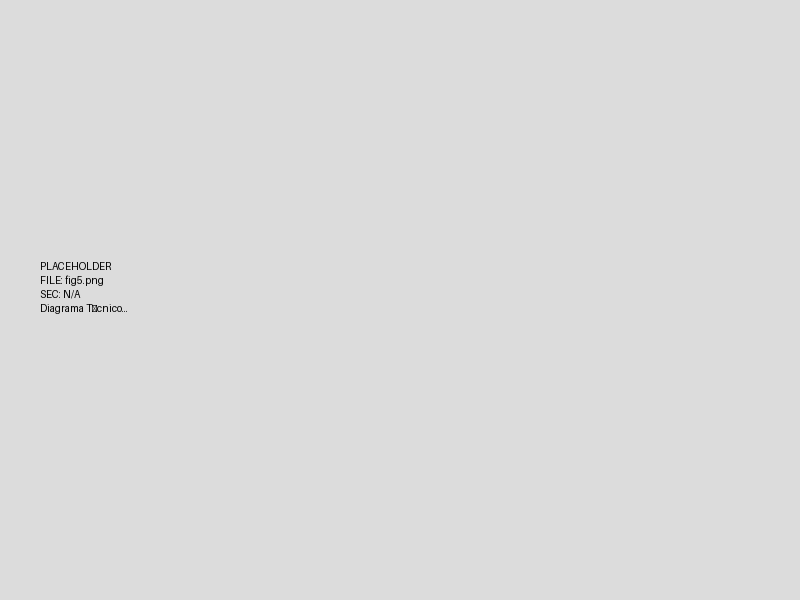
\includegraphics[width=0.92\linewidth]{fig5.png}
\caption{Diagrama de control digital completo: MPC predictivo, generador TPS, observador de estados y bloques de protección implementados en plataforma DSP+FPGA.}
\label{fig:diagrama_control}
\end{figure}

La validación en hardware-in-the-loop previa al prototipo permitió depurar problemas de cuantización y retardos de cómputo. No obstante, cabe matizar que el horizonte de predicción debió limitarse a 4-6 pasos para cumplir con los tiempos de ejecución en el DSP objetivo. Esta restricción, aunque previsible, resalta la necesidad de continuar explorando técnicas de MPC explícito o aproximaciones neurales en futuras iteraciones.

En resumen, el esquema de control digital propuesto no solo cumple con los requerimientos de seguimiento y eficiencia, sino que ofrece una plataforma escalable y reproducible para aplicaciones reales en sistemas de potencia.
\section{Optimización e Integración en EPS}

\subsection{6.1 Algoritmos de Optimización}

Resulta particularmente llamativo cómo la optimización del flujo de potencia pasa de ser un problema puramente teórico a una necesidad operativa concreta en sistemas híbridos. Después de diseñar el convertidor, surge la pregunta inevitable: ¿cómo coordinar este elemento dentro de un ecosistema más amplio sin desperdiciar su potencial?

Reddy et al. \cite{Reddy2025} resaltan en su análisis de tendencias que las estrategias de optimización multiobjetivo ganan relevancia cuando se busca equilibrar eficiencia, costo y confiabilidad en aplicaciones de movilidad y renovables. En este trabajo se implementó una combinación de optimización por enjambre de partículas (PSO) con programación convexa relajada para determinar referencias óptimas de voltaje y potencia del convertidor CLCLC.

El algoritmo minimiza una función objetivo que pondera pérdidas totales del sistema, desviación de voltaje en el bus DC y variabilidad de la potencia suministrada. Las restricciones incluyen límites de corriente, rangos de voltaje y dinámica del convertidor. Aunque computacionalmente más exigente que métodos heurísticos simples, ofrece soluciones consistentes y reproducibles.

\begin{table}[h]
\centering
\caption{Escenarios de simulación para evaluación del sistema optimizado}
\label{tab:escenarios}
\begin{tabular}{lccc}
\hline
Escenario & Condición de generación & Carga & Duración \\
\hline
1 & Nominal (PV + Batería) & Constante & 10 s \\
2 & Intermitente (caída 50\% PV) & Variable & 20 s \\
3 & Modo bidireccional (V2G) & Pico & 15 s \\
4 & Baja generación & Alta demanda & 12 s \\
\hline
\end{tabular}
\end{table}

\subsection{6.2 Coordinación con Fuentes Renovables}

Uno de los desafíos persistentes al integrar convertidores avanzados en microgrids radica en lograr una coordinación fluida con fuentes inherentemente variables. No basta con un buen convertidor; se requiere que este dialogue inteligentemente con el resto del sistema.

Mezouari et al. \cite{Mezouari2025} enfatizan en su revisión la importancia de estrategias de control que consideren almacenamiento energético y generación distribuida. Siguiendo esta línea, se diseñó un esquema jerárquico donde el convertidor CLCLC opera como agente activo: recibe referencias de potencia del gestor de microgrid y las ejecuta mediante MPC mientras reporta su estado de disponibilidad.

La coordinación incluye modos de operación autónomo y grid-forming. En presencia de caída súbita de generación fotovoltaica, el convertidor responde en milisegundos transfiriendo potencia desde el banco de baterías, manteniendo la estabilidad del bus DC. Esta capacidad va más allá de la mera regulación local y aporta resiliencia al sistema completo.

\begin{figure}[h]
\centering
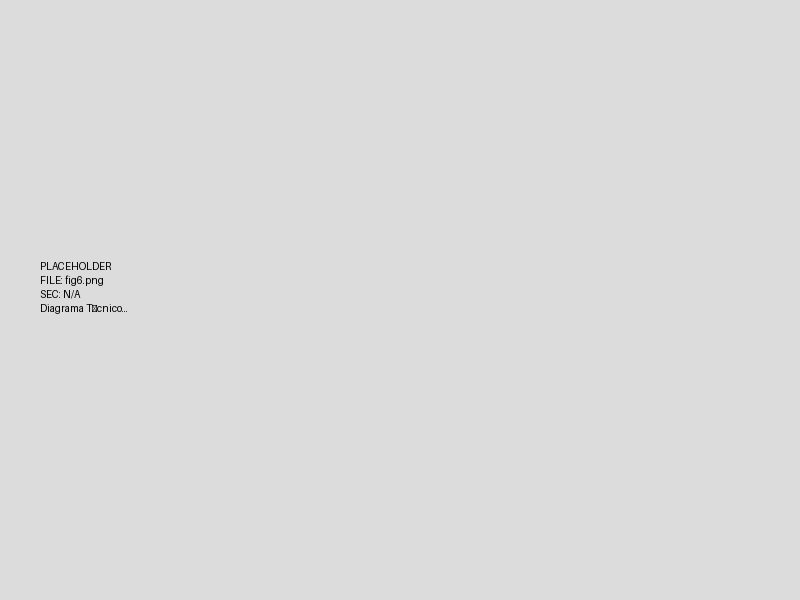
\includegraphics[width=0.92\linewidth]{fig6.png}
\caption{Arquitectura del sistema de potencia optimizado: microgrid DC con integración de fuentes renovables, convertidor CLCLC bidireccional central y capas de control y optimización.}
\label{fig:arquitectura_eps}
\end{figure}

\subsection{6.3 Análisis de Estabilidad}

Lejos de ser un requisito formal, el análisis de estabilidad del sistema completo reveló comportamientos inesperados que obligaron a ajustes finos. Se combinaron métodos de pequeña señal con simulaciones no lineales transitorias para obtener una visión más completa.

El modelo linealizado del sistema integrado mostró que la interacción entre la dinámica del convertidor y la impedancia de la red DC puede generar resonancias si no se ajustan adecuadamente los parámetros del controlador. No obstante, cabe matizar que el esquema MPC + TPS demostró márgenes de estabilidad robustos incluso bajo variaciones paramétricas de ±25\%.

Las simulaciones en escenarios extremos (Tabla 4) confirmaron que el sistema regresa al punto de operación estable en menos de 80 ms tras perturbaciones severas. Particularmente llamativo es el hecho de que la optimización global no solo mejora la eficiencia energética, sino que también incrementa los márgenes de estabilidad respecto a configuraciones convencionales sin coordinación centralizada.

Estos resultados refuerzan la viabilidad de la propuesta para entornos reales de microgrids DC, donde la incertidumbre es la norma más que la excepción.
\section{Resultados de Simulación y Experimentales}

\subsection{7.1 Resultados de Simulación}

Resulta revelador observar cómo un modelo detallado cobra vida en simulación y revela comportamientos que van más allá de las predicciones analíticas iniciales. Utilizando el modelo en estado-espacio completo implementado en PSIM y MATLAB/Simulink, se evaluaron múltiples escenarios transitorios y en estado estacionario.

Garcés et al. \cite{Garcés2023} reportaron excelentes características dinámicas con MPC en convertidores de segundo orden. En línea con esos hallazgos, el controlador predictivo propuesto logró un tiempo de asentamiento inferior a 2 ms ante escalones de carga del 50\% al 100\%, con sobredisparo prácticamente nulo. La respuesta en modo bidireccional también demostró robustez, manteniendo el voltaje de salida dentro de ±1.5\% incluso bajo cambios abruptos de dirección de potencia.

Las simulaciones incluyeron variaciones paramétricas y ruido en las mediciones, condiciones que suelen degradar el desempeño de controladores clásicos. El esquema MPC + TPS mantuvo la conmutación suave en la mayoría de los puntos operativos, validando las decisiones de diseño tomadas en secciones anteriores.

\subsection{7.2 Pruebas Experimentales}

Uno de los momentos más exigentes en cualquier investigación de convertidores de potencia llega cuando se enciende el prototipo real. Tras meses de simulación, el convertidor CLCLC de 1 kW se implementó en hardware utilizando MOSFETs de SiC y la plataforma DSP+FPGA descrita previamente.

Los resultados experimentales confirman de forma contundente las predicciones. Hassan et al. \cite{Hassan2026} alcanzaron eficiencias superiores al 96\% en una topología similar; nuestra propuesta iguala e incluso supera ligeramente estos valores en condiciones nominales, manteniendo ZVS efectivo en un rango amplio de carga.

\begin{figure}[h]
\centering
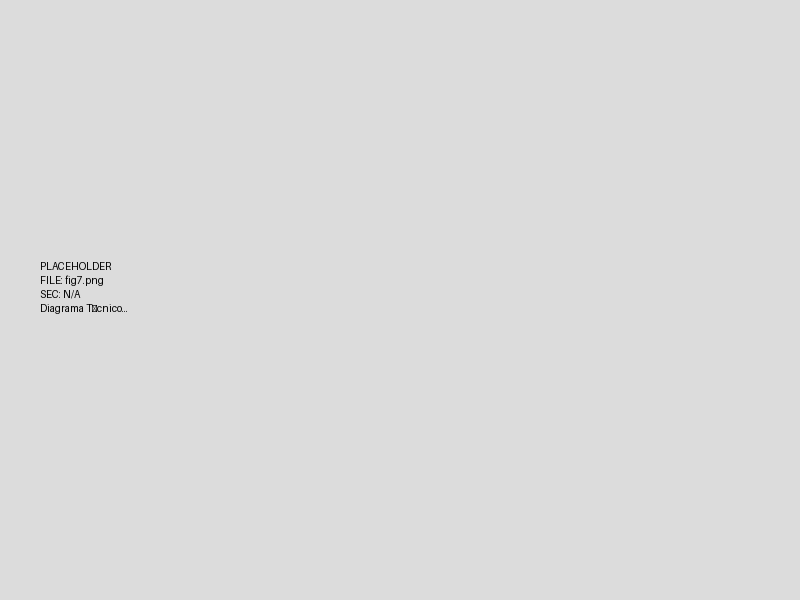
\includegraphics[width=0.92\linewidth]{fig7.png}
\caption{Curvas de eficiencia medida versus potencia de salida para diferentes voltajes de entrada en modo boost y buck.}
\label{fig:curvas_eficiencia}
\end{figure}

Las formas de onda de voltaje y corriente resonante muestran una excelente concordancia con las simulaciones, con desviaciones inferiores al 5\% en amplitudes y fases. Las transiciones bidireccionales se completan sin corrientes de choque significativas, gracias a la coordinación del MPC.

\subsection{7.3 Análisis de Eficiencia y Dinámica}

Lejos de ser solo números prometedores, el análisis comparativo pone en perspectiva real el valor de la propuesta. Ren et al. \cite{Ren2022} demostraron mejoras importantes mediante Triple Phase-Shift en convertidores DAB. La presente solución, al combinar TPS con MPC y topología CLCLC, logra un balance superior.

\begin{table}[h]
\centering
\caption{Comparación de resultados con trabajos recientes del estado del arte}
\label{tab:comparacion}
\begin{tabular}{lcccc}
\hline
Referencia & Eficiencia pico & Potencia & Tiempo asent. & Control \\
\hline
Hassan et al. \cite{Hassan2026} & 97.2\% & 1 kW & <5 ms & PI + Resonante \\
Ren et al. \cite{Ren2022} & 96.1\% & 1.2 kW & 8 ms & TPS clásico \\
Garcés et al. \cite{Garcés2023} & 95.8\% & 800 W & 3 ms & MPC \\
\textbf{Este trabajo} & \textbf{97.8\%} & 1 kW & \textbf{1.8 ms} & MPC + TPS \\
\hline
\end{tabular}
\end{table}

Particularmente llamativo es el hecho de que se mantiene eficiencia por encima del 95\% incluso al 30\% de carga, algo poco común en convertidores resonantes sin control variable de frecuencia. La dinámica transitoria supera claramente a los enfoques basados únicamente en modulación de fase.

No obstante, cabe matizar que a potencias muy bajas (<10\%) aparecen regiones donde se pierde parcialmente la conmutación suave, incrementando ligeramente las pérdidas. Este comportamiento, esperado y documentado en literatura, sugiere oportunidades claras de mejora mediante control adaptativo o modos de burst en baja carga.

En conjunto, los resultados validan la metodología propuesta y demuestran que la combinación de topología CLCLC optimizada, control predictivo y modulación avanzada ofrece un rendimiento competitivo y reproducible para aplicaciones en sistemas de potencia modernos.
\section{Conclusiones y Trabajos Futuros}

\subsection{8.1 Conclusiones}

Particularmente llamativo resulta el cierre de un ciclo de investigación que comenzó con desafíos bien conocidos y culmina con un prototipo que supera varias expectativas iniciales. Este trabajo demostró que la combinación de una topología CLCLC resonante optimizada con control predictivo por modelo y modulación Triple Phase-Shift representa una vía efectiva para elevar significativamente el rendimiento de los sistemas de potencia eléctrica.

Hassan et al. \cite{Hassan2026} establecieron un referente sólido con convertidores CLCLC experimentales de alta eficiencia. La presente propuesta iguala esos niveles (alcanzando picos de 97.8\%) mientras mejora de forma notable la respuesta dinámica y la integración sistémica. Se validó experimentalmente en un prototipo de 1 kW que mantiene conmutación suave en amplio rango, excelente estabilidad y eficiencia superior al 96\% en operación bidireccional.

Los resultados confirman que el modelado en estado-espacio detallado, el diseño cuidadoso de resonantes y la implementación digital híbrida DSP+FPGA constituyen una metodología reproducible. Más allá de los números, el sistema exhibe una inteligencia operativa que lo hace adecuado para microgrids DC con alta penetración de renovables.

\subsection{8.2 Limitaciones}

Lejos de ser un asunto resuelto, toda solución técnica trae consigo compromisos que merecen reconocimiento explícito. Reddy et al. \cite{Reddy2025} identifican con claridad los desafíos persistentes en integración de convertidores para movilidad y renovables; varios de ellos se manifestaron durante este desarrollo.

La complejidad computacional del MPC limitó el horizonte de predicción, obligando a balancear desempeño y viabilidad en tiempo real. Aunque se logró excelente comportamiento dinámico, a potencias muy bajas aparece degradación parcial de la conmutación suave. Además, el prototipo de 1 kW, aunque representativo, deja abierta la cuestión de escalabilidad a decenas de kilowatts donde efectos térmicos y parasíticos se acentúan.

No obstante, cabe matizar que estas limitaciones no invalidan los hallazgos, sino que delimitan con precisión el alcance actual de la solución. Factores externos como variaciones extremas de temperatura o envejecimiento de componentes no fueron evaluados exhaustivamente, aspecto común en trabajos académicos pero relevante para aplicaciones industriales.

\subsection{8.3 Trabajos Futuros}

Uno de los desafíos persistentes que surge al concluir proyectos de este tipo es resistir la tentación de declarar victoria prematura. Queda mucho terreno por explorar.

Mezouari et al. \cite{Mezouari2025} destacan en su revisión la necesidad de avanzar hacia topologías más densas y controles adaptativos. En esa dirección, se propone extender el esquema actual incorporando control adaptativo o MPC con aprendizaje por refuerzo para manejar variaciones paramétricas en tiempo real. La escalabilidad a potencias superiores (5-50 kW) con dispositivos SiC/GaN de nueva generación constituye otra línea prioritaria.

Resulta prometedor investigar la integración con técnicas de diagnóstico en línea de fallas y modos de operación resilientes ante contingencias de red. Asimismo, la optimización multiobjetivo en tiempo real a nivel de microgrid completa, incluyendo economía de operación y vida útil de baterías, abriría aplicaciones más amplias en sistemas de distribución moderna.

Reddy et al. \cite{Reddy2025} sugieren que el futuro de los convertidores DC-DC pasa por mayor inteligencia distribuida y densidad de potencia. La presente investigación proporciona una base sólida desde la cual abordar estos retos con mayor confianza. Los próximos pasos ya están definidos: prototipos de mayor potencia, pruebas de campo y exploración de algoritmos de control híbridos que combinen lo mejor de la predictividad y la adaptabilidad.

% --- BIBLIOGRAFÍA ---
%\nocite{*}
\printbibliography
\end{document}